\documentclass[twoside,10pt]{article}
\usepackage{multicol,graphicx,caption,cite}
\usepackage{amsmath,fouriernc,parskip,amssymb}
\usepackage[top=.5in,bottom=.5in,left=.5in,right=.5in,columnsep=20pt]{geometry}
\setlength{\parindent}{2em}
\setlength{\parskip}{0em}

\title{CS6490 Project Report: Multiple Service Authentication Protocol}
\author{Jeff Brock, Roozbeh Gholizadeh, Montgomery Carter}
\date{}

\newenvironment{Figure}
  {\par\medskip\noindent\minipage{\linewidth}}
  {\endminipage\par\medskip}

% Determine if the image is too wide for the page.
%\def\ScaleIfNeeded{%
%  \ifdim\width>\linewidth
%    \linewidth
%  \else
%    \width
%  \fi
%}

%\let\origincludegraphics\includegraphics
%\renewcommand*\includegraphics[2][]{%
%    \resizebox{\ScaleIfNeeded}{!}{\origincludegraphics[#1]{#2}}%
%}

\begin{document}
\maketitle
\newpage
\begin{multicols}{2}

\section{Introduction}
We rely on large tech organizations more and more to facilitate our daily communication.  As a result, these large tech organizations have access to our personal information, from the mundane to the deeply personal and revealing.

While operating off the grid may work for some individuals, the convenience of such services provides a compelling argument in favor of their use.  The typical attitude is to accept the loss of privacy in exchange for use of the service.  Rather than forgoing the convenience of utilizing these services, or acquiescing our privacy, it is desirable to have a solution that protects our privacy as we use these services.

In this paper, we focus on instant messaging (IM) communication because it is a real time communication that allows the exchange of messages to establish privacy for the duration of a conversation.  Our proposed solution could easily be extended to email services, though it seems more natural in the context of real time communications.  There are many solutions to provide a layer of authentication and encryption that run on top of such services as Google Hangouts, Facebook Chat, Skype, etc.  However, these solutions are complicated, and generally rely on an external authentication service \cite{DiRaimondo:2005:SOM:1102199.1102216}, or public-key (RSA, DSA, PGP) based authentication to establish shared session keys for encrypting and integrity protecting the ensuing communication.  Configuring such a solution is complex enough to dissuade the typical user from employing them, and can have cost associated that provides further barrier to use.

It would be desirable to have a method for encryption and integrity protection that does not require external authentication (which means an additional service to trust), and does not use complicated public key signature schemes for integrity protection.

We present the Multiple Service Authentication Protocol (MSAP), a protocol for establishing shared session keys to be used for encryption and integrity protection of instant messaging (IM) communications. Unlike existing solutions, MSAP does not, itself, rely on public key authentication.  Instead, MSAP relies on using more than one service at a time, including the authentication performed by service providers such as Google, Microsoft, or Facebook to verify the identities of IM conversation participants.  IM service providers have an incentive to deliver messages to the intended recipient, as well as to ensure that only the intended recipient has access to delivered messages.  Without this, their service is of little use and they would have no user base.  To ensure these criteria, an IM service must authenticate users.

Further, the protocol ensures that service providers do not have access to the shared session keys, and importantly, prevents service providers from employing a man in the middle (MitM) attack and acting as an interfering intermediary between the two communicating parties.

Unsurprisingly, MSAP utilizes a Diffie-Hellman (DH) key exchange for the establishment of shared session keys \cite{diffie1976new}.  The more interesting feature of MSAP is its use of multiple, separate messenger services to perform the requisite DH exchange.  By sending half of the DH exchange via one IM service, and the response via a separate IM service, no one service is privy to both sides of the exchange, rendering both services incapable of mounting a MitM attack.

Although the main goal of protecting against MitM attacks from service providers is achieved simply by moving the DH response to a separate service, there is still a threat of MitM attacks from an external intruder who may have control of some node on the route between communicating parties, and is able to modify messages between one participant and multiple chat services. To address this threat, MSAP includes two mechanisms to protect against MitM attacks performed by external parties (e.g., one chat participant's ISP network).  The first (and preferable) mechanism works by requiring SSL encryption between chat client and chat host (which is available with many IM providers such as Facebook and Google) for at least one of the DH exchange messages.  By using SSL in this manner, such an intruder will not have all of the information necessary to mount an MitM attack.

If no chat service offering SSL encryption is available, the second mechanism comes in to play, where each participant remembers a temporary ``long term'' secret (TLTS).  This temporary ``long term'' secret is used in lieu of a DH exchange to encrypt the exchange of the session keys for every conversation subsequent to the initial conversation between the two parties.  During each subsequent conversation between the parties, this TLTS is updated with a new TLTS.  Of course, this assumes that no intruder performs an MitM attack during the initial conversation.

\section{Related Work}
Existing solutions for encrypting IM communications generally take the same form.  They generally require users to utilize RSA, DSA, PGP, or some other method of public key signatures.  For authentication, this requires registration with a certificate authority, which incurs cost, or a less secure chain of trust in the case of PGP.  While a registered public key signature method is probably the most secure, it requires significant knowledge and some cost to implement.  This is likely out of reach for a majority of IM users, particularly the less technically minded.  We were unable find a scholarly article about such solutions, but one example is the Pidgin-Encryption plugin (http://pidgin-encrypt.sourceforge.net/) for the multi-service chat client, Pidgin \cite{PidginEncryption}.  

Another popular solution is the Off-The-Record (OTR) protocol, which uses certificates or other mechanisms for authenticating users and negotiating shared session keys \cite{DiRaimondo:2005:SOM:1102199.1102216}.  It does include some more interesting options than just using public key certificates, such as creating a security question that supposedly only the other user would know, however this is less secure.  This solution is widely implemented, however it requires user be aware of it, understand the methods of the protection, and to configure it.

%Our proposal requires only that users understand their communications are protected if they have more than one IM service available.
Finally, we rely on the very frequently cited work of Diffie and Hellman \cite{diffie1976new}.  There is nothing new here - this is the standard DH exchange protocol.  However, by authenticating using the IM service providers, we avoid having to do authentication ourselves.

\section{Adversary Model}
In our adversary model we assume two nefarious players.  The relationship between these players and the chat participants are only described for Alice, however, apply equally well to Bob.

The first is Hank the host, the server hosting a chat service.  We assume Hank securely and accurately authenticates users, however is motivated to read communications in order to build behavioral models and sell ads (or perhaps more sinister reasons).  Hank is capable of mounting a MitM attack on a DH exchange conducted exclusively over a single chat service, as he necessarily must receive and relay all messages between Alice and Bob.  Even when encryption is used between client and server, as the server Hank still has access to read and modify (or replace) the plaintext messages between participants.  We refer to this type of attack as an internal MitM attack.  Hank, however, doesn't  control any node that sits on the route between Alice and multiple chat services (including Hank).  It is conceivable that Hank may have control of a few nodes in his periphery network, but not some node that allows Hank to modify messages between Alice and some other chat service.  Further, we assume that there is no collusion between IM services where Hank may begin an MitM attack, and inform the second service that a DH exchange is occurring, and what the first half of the MitM attack keys are.

Trudy has control of some node along the route that is between Alice and every chat service (perhaps Trudy is Alice's ISP), and is capable of performing a MitM attack.  We refer to this more traditional type of MitM attack as an external MitM attack.

We assume that both Hank and Trudy know MSAP, as well as the encryption and message digest algorithms used by MSAP.

In short, we consider the chat service providers to be capable of modifying messages only as they relay them, and external intruders capable of modifying any message sent/received to one of the chat participants.  

\section{Protocol Definition}\label{sec:protoDef}
In this section we first introduce some terminology and bookkeeping.  Let $S$ be a list of chat services.  Alice maintains a list of usernames for Bob, $U_{B}$, where each $U_{B_x}$ is Bob's username for $S_x$.  Bob maintains a similar list, $U_{A}$, for Alice.  Alice and Bob also keep track of a temporary ``long term'' secret, $TLTS_{AB}$.  Encryption and integrity protection algorithms between Alice and Bob can be any accepted, secure algorithm.  Let $f(a,b)$ be a secure function for generating a session key based on two input nonces.  Let $g(a,b)$ be a second secure function for generating a key, where $f(a,b) \neq g(a,b)$, and the output of $f(a,b)$ cannot be predicted from $g(a,b)$, and vice versa.

MSAP is described below, with Alice initiating communication with Bob
\begin{enumerate}
\item Alice and Bob both sign in to $S_0$, with encryption required between client and host.
\item If $TLTS_{AB}$ is defined, Alice chooses a nonce, $N_0$ and a next service, $S_n$ where $S_n \neq S_0$, and sends $\{U_{B_0}, TLTS_{AB}\{N_0\}\}_{SSL S_0 A}$ to $S_0$, which relays $\{TLTS_{AB}\{N_0\}, S_n\}_{SSL S_0 B}$ to Bob.  If $TLTS_{AB}$ is undefined, proceed to step \ref{wbp:beginDH}.
\item Bob sends $\{U_{A_0}, TLTS_{AB}\{N_0-1\}\}_{SSL S_0 B}$ to $S_0$, which relays $\{TLTS_{AB}\{N_0-1\}\}_{SSL S_0 B}$ to Alice.
\item If Bob's response decrypts to $N_0-1$, both parties set $DH_{AB}:=TLTS_{AB}$, and continue with step \ref{wbp:beginDH}, but encrypt all subsequent protocol messages with $TLTS_{AB}$.  If not, abort authentication.
\item \label{wbp:beginDH} Alice chooses a DH base $g$, modulus $p$, and secret exponent $a$, as well as a next service, $S_n$ where $S_n \neq S_0$.
\item Alice sends $\{U_{B_0}, p, g^a mod p, S_n\}_{SSL S_0 A}$ to $S_0$, which relays $\{g, p, g^a mod p, S_n\}_{SSL S_0 B}$ to Bob.
\item Alice and Bob both sign in to $S_n$.  (Encryption unimportant)
\item Bob selects a DH secret exponent $b$.
\item Bob sends $\{U_{A_n}, g^b mod p\}_{SSL S_0 B}$ to $S_0$, which relays $\{g^b mod p\}_{SSL S_0 A}$ to Alice.
\item Alice and Bob both calculate $DH_{AB}:=g^{ab} mod p$.
\item \label{wbp:beginNonceExchange} Alice and Bob choose nonces, $N_A$ and $N_B$
\item Alice sends $DH_{AB}\{N_A\}$ to Bob, and Bob sends $DH_{AB}\{N_B\}$ to Alice, both via $S_n$.
\item Alice and Bob both calculate the session key, $K_{AB}=f(N_A, N_B)$
\item Both Alice and Bob calculate and update $TLTS_{AB}=g(N_A, N_B)$.
\end{enumerate}

MSAP is summarized in Figure~\ref{fig:fullProto}.


\begin{Figure}
  \centering
  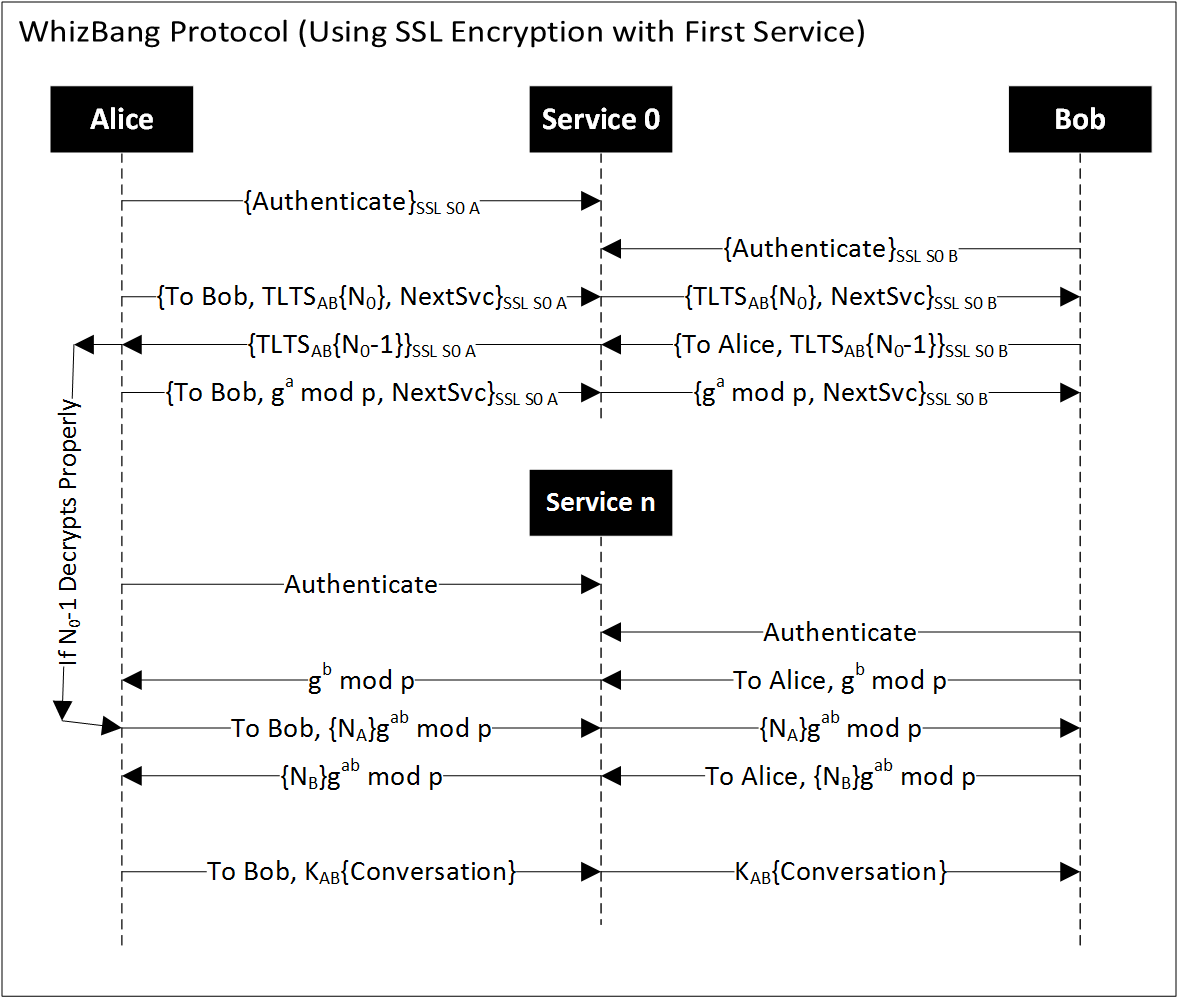
\includegraphics[width=\linewidth]{ProtocolDiagramBW}
  \captionof{figure}{MSAP with $TLTS_{AB}$ pre-established}\label{fig:fullProto}
\end{Figure}


\section{Discussion}
Because we assume IM services faithfully perform authentication and message delivery, we know a message destined for Bob via $S_0$ will reach Bob.  However, if $S_0$ notices a DH exchange occurring, it may opt to begin an MitM attack, and deliver a separate DH exchange for which it knows the DH exponent.  To protect against this internal MitM threat, it is sufficient to simply complete the DH exchange on a separate service, as illustrated in Figure~\ref{fig:basicProto}.
\begin{Figure}
  \centering
  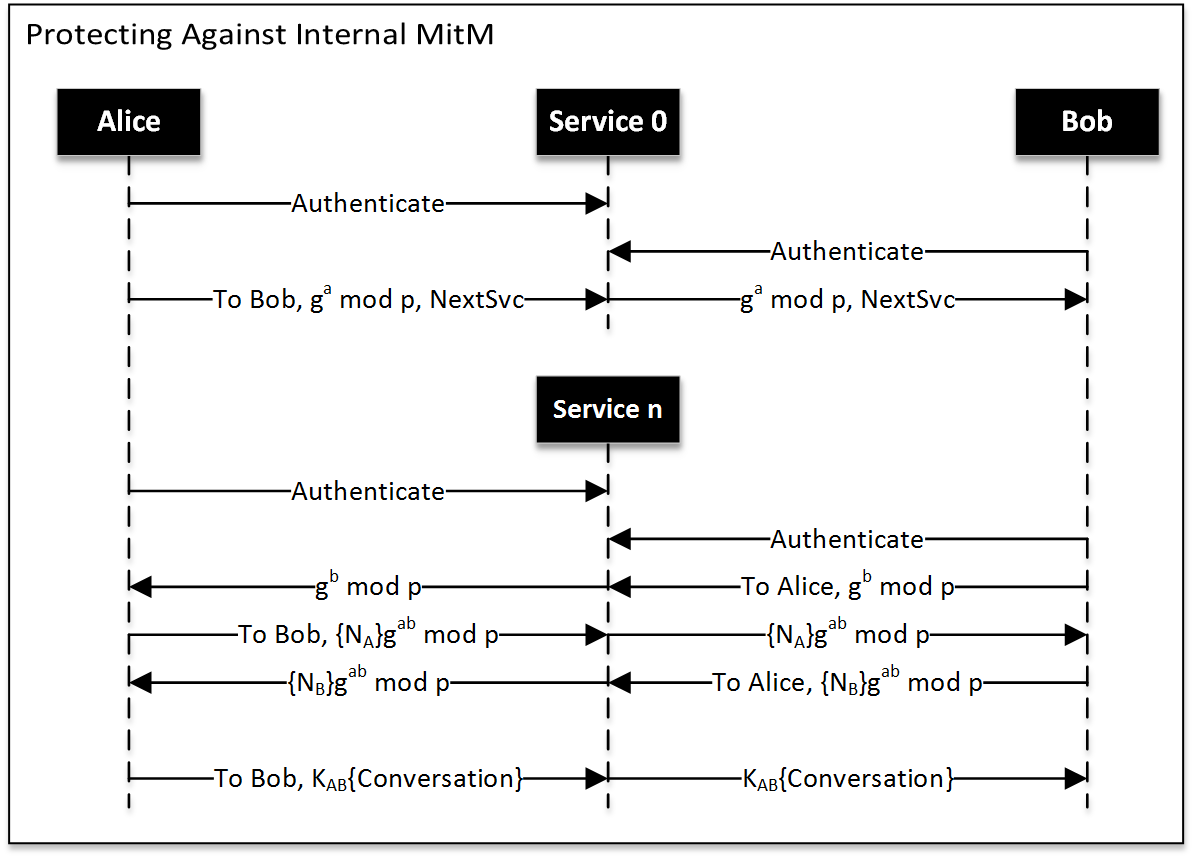
\includegraphics[width=\textwidth]{ProtectInternalMitMDiagramBW.png}
  \captionof{figure}{Protecting Against Internal MitM}\label{fig:basicProto}
\end{Figure}

Because the initiating party is not listening for a DH key exchange response on $S_0$, any MitM response from $S_0$ to the initiating party is disregarded.  This prevents this hosting server from performing an MitM.  Similarly, because no party is listening for a DH exchange response on $S_n$, there is no opportunity this service to perform an MitM attack (Note that always choosing $S_0$ for the first exchange is sent is only for ease of discussion.  Any service in $S$ may be used for the first message, so long as it is different than $S_n$).

Having established a DH shared key, Alice and Bob can now exchange nonces that can be used to generate shared session keys for the encryption and integrity protection algorithms of their choice.

Still, this leaves opportunity for an external MitM attack.  If an adversary has control of part of the route to one of the participants, such attack is still feasible, using only the protocol described by Figure~\ref{fig:basicProto}.  To address this concern, MSAP employs two strategies for addressing this vulnerability.

The first, and preferred, strategy is to use an IM service that normally performs encryption between the participants and the IM service host for at least one direction of the DH exchange.  This mechanism is illustrated in Figure~\ref{fig:sslProto}.

By wrapping the initial DH message from Alice to Bob in SSL established between Alice and $S_0$, any attempt by Trudy to mount an MitM is thwarted, as SSL provides encryption and message authentication.  As a result, it is impossible for Trudy to learn $g^a mod p$.  This means that even if she is capable of modifying messages between Alice and all other IM servics including $S_n$, the best she can do is make Alice and Bob disagree on $g^{ab} mod p$.  Note that this protection is also afforded when $S_0$ is not encrypted, but $S_n$ is.

\begin{Figure}
  \centering
  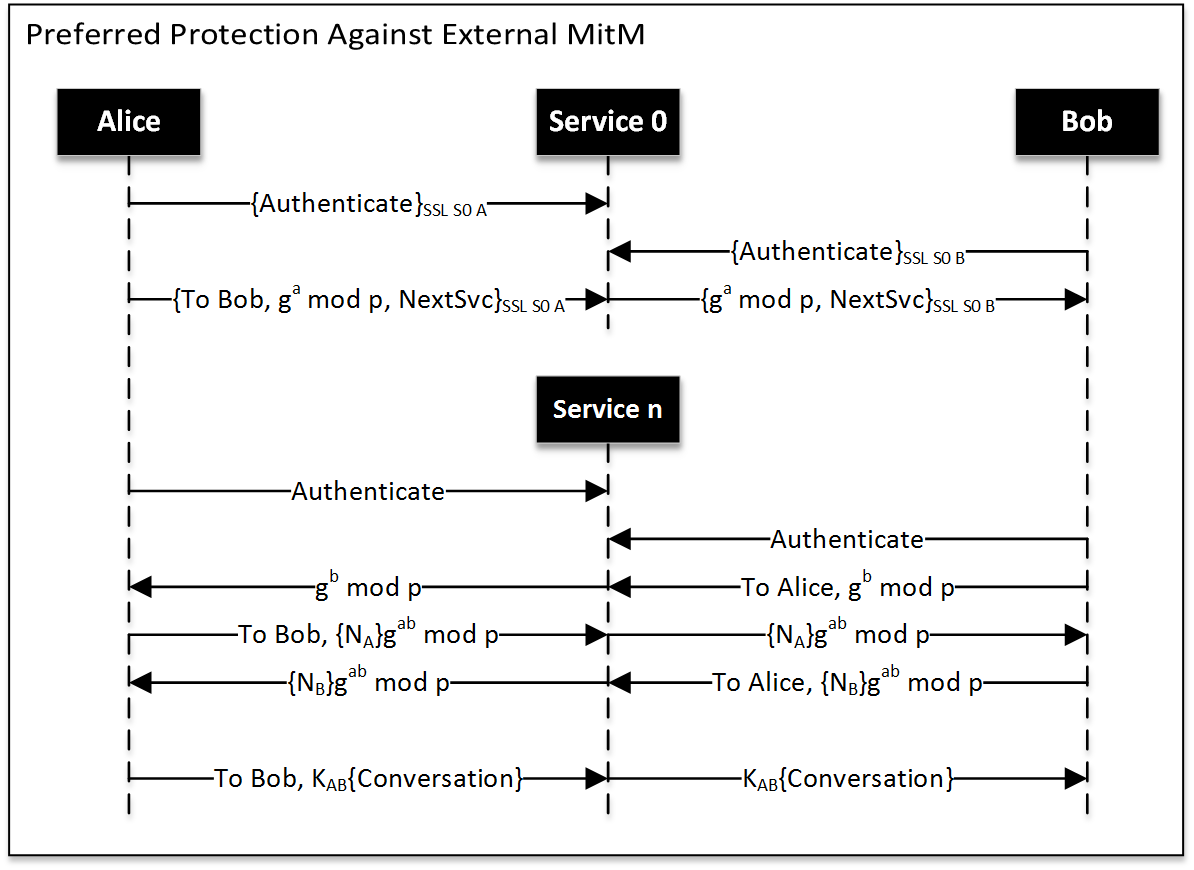
\includegraphics[width=\textwidth]{SSLOnlyDiagramBW.png}
  \captionof{figure}{Preferred Protection Against External MitM}\label{fig:sslProto}
\end{Figure}

In the event that no IM provider offering SSL is available (or preferred by the participants), the second strategy is employed to exchange a temporary ``long term'' key between parties, which is then used to encrypt the DH exchange of subsequent conversations between the same parties.  However, this second strategy assumes that an intruder was not present during the \emph{initial} conversation between the parties (otherwise an intruder would know the temporary long term key).  This temporary ``long term'' key is replaced after the DH key exchange of each conversation between the parties.  This requires an intruder to be  present for \emph{every} conversation between the parties, as missing a conversation means the temporary ``long term'' key they knew has been replaced without them being able to observe the replacement.

Although mechanism 1 and 2 can be used independently to protect against external MitM attacks, the final version of the protocol, as defined in Section~\ref{sec:protoDef}, calls for both to be used together, where possible.  This allows for the secure establishment of a TLTS during a first SSL-encrypted session, addressing the assumption that no intruder is present during this initial conversation.  Subsequent conversations are then free to perform MSAP over unencrypted connections between client and host.

Note that these ambiguities in the protocol allow for a user-configurable level of protection.

\section{Implementation}
To demonstrate the functionality of MSAP, we developed a proof of concept implementation.  Our prototype is written in Python, and utilizes an XMPP chat protocol implementation from the Twisted library \cite{TwistedHomepage}.  Our implementation can be found in the GitHub repository, https://github.com/cs6490groupJMR/ProtoSecureChat.

As we developed this proof of concept, we found that MSAP is trivial to add to any multi-service chat client.  The proof of concept is very basic, however it is able to show how MSAP interacts with a normal XMPP chat service.  We were able to properly perform the DH exchange and encrypt messages, and we can see that the outgoing messages are protected from the chat service.

\section{Conclusion}
MSAP offers a much easier and more streamlined method for achieving privacy and integrity protection on top of publicly available IM services such as Google Hangouts, Facebook Chat, Skype, etc.  By requiring only that users have accounts with more than one IM service, MSAP can ensure that these services are not able to read or modify the contents of conversations.  This is a much lower barrier than requiring the trust of a 3rd party authentication service, or the configuration of public key signature solutions.

Further, by utilizing the SSL encryption offered by many major IM service providers, MSAP ensures that external intruders capable of modify messages between the client and all chat services are unable to mount an MitM attack.  When SSL is not available with a client's preferred IM service, the secondary protection of using a TLTS is employed to thwart external MitM attacks.

Finally, we have demonstrated that deploying this solution to existing multi-service chat clients is trivial, and requires no modification of any underlying chat service protocols.  In fact, MSAP can be leveraged for non-IM communications such as email, by simply performing the MSAP message sequence via a standard email exchange.

\section{Appendix A: Protocol Extensions}
There are number of ways that MSAP can be extended to add interesting functionality.  

If we extend our adversary model to include collusion between multiple IM services, it is then possible for $S_0$ to do the first half of an internal MitM attack, and then provide the first half of the DH MitM exchange to $S_n$ alerting it that the second half of the DH exchange will be performed on their network.  $S_n$ now has sufficient information to complete a DH MitM attack.

With a two party chat, additional DH exchanges over different services can be chained together to increase the number of service providers that would have to collude in order to mount an internal MitM attack.  For example, after sending $g^a mod p$ and $g^b mod p$ over two services, the parties could then pick a third and fourth service, and send $g^c mod p$ and $g^d mod p$ over these services.  The DH secret key would then become $g^{abcd} mod p$, and require collusion between 4 chat services to mount an internal MitM attack.


MSAP can also be trivially extended to work with group chats, in addition to one-on-one chats.  This would work by simply creating a group DH exchange.  For example, Alice sends her DH public key to all participants on $S_0$.  All other participants, say Bob, Charlie, and Daphny, send their DH public keys to each other via $S_n$.  The DH shared secret then becomes $g^{abcd} mod p$.  This is identical to the concept of a group DH secret established over a single channel, except a second service is used to send the DH responses.  Because neither $S_0$ or $S_n$ hear all 4 DH public keys, an internal MitM attack is not possible services (assuming no collusion between service providers).

\section{Appendix B: Username Syncing}
It is purposeful that MSAP does not include any method for syncing usernames.  Usernames must be communicated outside of the protocol, as doing so allows $S_0$ to provide a username to an account that it controls with $S_n$.  This should obviously be avoided.

In general, the exchanging of usernames is a point of weakness in the protocol.  Even if done outside of the protocol, but within an IM conversation, if $S_0$ recognizes that Alice is sending Bob her username for $S_n$, it can switch out the username she provides with the username of an account that $S_0$ controls.

A method for securely exchanging usernames is outside the scope of this protocol, however clearly an out-of-band method such as in-person exchange or a phone call, would be sufficient for everyone except the most paranoid.  We do propose one alternative way of syncing usernames, provided Alice and Bob know each others usernames for two services.  The unknown usernames can be sent during the protocol by requesting a list of unknown usernames \emph{after} encryption is in place.  For example, if Alice is missing Bob's Facebook chat username, the protocol can be extended to send a message encrypted using $TLTS_{AB}$ to Bob via $S_n$, requesting his username for those services.

\bibliographystyle{plain}
\bibliography{ProjectReport}

\end{multicols}
\end{document}
